\section{Further \rib Details }
\subsection{Dataset List}
Table~\ref{tab:list_of_datasets} shows all datasets we used in \rib. Table~\ref{tab:refeences} provides references for these datasets. 
% \textcolor{red}{
% We use the following datasets for model training. 
% }

\subsection{Details of Dataset Unification}
\label{sec:unification}
As shown in Table~\ref{tab:list_of_datasets}, some datasets were not originally retrieval datasets (e.g., summarization datasets). 
We describe how we convert these into the unified retrieval task format. 

\paragraph{QA.}
For QA datasets, where each instance consists of a query, a gold context, and answers, we assume the original gold context as the gold document used as a positive sample during training. 
For some exceptional datasets, we performed additional preprocessing. 
We found that ReCoRD instances are occasionally self-containing due to the nature of the cloze-style QA; therefore, for ReCoRD, we replace the original placeholder with the gold answer and use this original question with the answer as the query and the original context as a gold document. 
For MedMCQA, we use the source exam question as the query and the answer evidence as the positive document. 

\paragraph{Summarization.}
For summarization datasets, we use target summarizations as the gold document and source text as the query. 

\paragraph{Text simplifications.}
For text simplification datasets, we use source (often more complex) sentences as the query and simplified sentences as the gold document. 

\paragraph{Code search.}
We use the source comment as the query and the corresponding implication as the gold document. We exclude the python subset from \rib as we use it for \task.  


\begin{table*}[ht!]
\center
\small
\begin{tabular}{l   c  c  c}
\toprule 
dataset & domain & task & unit\\\midrule
1. Altlex & Wikipedia & sentence paraphrase & sentence \\ 
2. StackExchange (title $\rightarrow$ title) & community forum & duplicated questions & title  \\ 
3. StackExchange  (query $\rightarrow$ answer) & community forum& QA & answer body  \\ 
4. Yahoo Answers (title $\rightarrow$ answers) & community forum &  QA & answer body  \\ 
5. MS MARCO & web &  QA & paragraph  \\ 
6. ELI5 & web &  QA & answer paragraph  \\ 
7. WikiHow & community forum &  QA & answer paragraph  \\ 
8. SearchQA & web &  QA & search snippets \\ 
9. AGNews & News &  summarization & news summary \\ 
10. NPR & News &  summarization & news summary \\ 
11. CodeSearchNet (java) & code & code search & Java code \\ 
12. CodeSearchNet (ruby) & code & code search & Ruby ode \\ 
13. CodeSearchNet (JavaScript) & code & code search & Java Script code \\ 
14. CodeSearchNet (Go) & code & code search & Go code \\ 
15. PAQ & Wikipedia & QA & paragraph \\ 
16. Sentence Compression & misc. & sentence compression & sentence \\
17. CNN Daily Mail & news & summarization & news summary \\
18. XSUM & news & summarization & news summary \\
19. Coco captions & image captions & caption generations & captions \\
20. Quora Duplicated Questions &  community forum & duplicated questions & questions \\
21. CCNews &  news & summarization & news summary  \\
22. FEVER  (KILT) &  Wikipedia & fact verification & paragraph  \\
23. HotpotQA  (KILT) &  Wikipedia & QA & paragraph  \\
24. NQ  (KILT) &  Wikipedia & QA & paragraph  \\
25. TriviaQA (KILT) &  Wikipedia & QA & paragraph  \\
26. WoW-KILT (knowledge) &  Wikipedia & knowledge-grounded dialogue & paragraph  \\
27. WoW-KILT (response) &  Wikipedia & knowledge-grounded dialogue & dialogue response  \\
28. medical simplification &  medical & sentence simplification & sentence  \\
29. SciTLDR &  science & summarization & paper summarization  \\
30. PubMedQA &  medical\& science & QA & abstract \\
31. MedMCQA &  medical & QA & answer explanation \\
32. Gigaword &  web & headline retrieval & headline \\
33. ReCoRD &  news &QA & news summary \\
34. MultiLexSum &  legal & summarization & legal case summary \\
35. Qrecc & Wikipedia & conversational QA & response \\
36. OQA & Wikipedia & duplicated questions & question \\
37. SQuAD & Wikipedia & QA & paragraph \\
\bottomrule
\end{tabular}
\caption{The complete list of datasets included in \rib.  Table~\ref{tab:refeences} shows references for them.
% In addition to the datasets listed above, we have data from CodeSearch-python and CodeSearch
}
\label{tab:list_of_datasets}
\end{table*}
\begin{table*}[t!]
\renewcommand{\arraystretch}{1.2}
\setlength{\tabcolsep}{2pt}
\footnotesize
    \centering
    \begin{tabular}{p{15cm}}%|ccccccc}
\toprule
%\sandy{Whoa. Akari...the following is very hard to parse and read. Can you list these rather than run them into the same paragraph? Also, can reader access the dataset using only this information? Further, list the following in the same order as you list the ones in Table 5 for ease of cross-matching.}
% {\bf Training} & \\
{\it datasets used in \rib} \\\hline
Altlex$^{*}$~\cite{hidey-mckeown-2016-identifying}, StackExchange (duplicate questions, question-title, question-question)~\cite{reimers2019sentence}, Yahoo Answers$^{*}$~\cite{yahoo_answers}, MSMARCO$^{*}$~\cite{msmarco}, ELI5$^{*}$~\cite{fan-etal-2019-eli5}, WikiHow$^{*}$~\cite{koupaee2018wikihow}, SearchQA$^{*}$~\cite{dunn2017searchqa}, AG News$^{*}$~\cite{agcorupus}, NPR$^{*}$~\cite{NPR}, CodeSearchNet$^{*}$~\cite{husain2019codesearchnet}, PAQ$^{*}$~\cite{lewis-etal-2021-paq}, Sentence Compression$^{*}$~\cite{filippova-altun-2013-overcoming}, CNN Daily Mail$^{*}$~\cite{see-etal-2017-get}, XSUM$^{*}$~\cite{narayan-etal-2018-dont}, COCO captions$^{*}$~\cite{chen2015microsoft}, Quora Duplicated Questions~\cite{quora}, CC News$^{*}$~\cite{Hamborg2017}, SQuAD$^{*}$~\cite{rajpurkar-etal-2016-squad}, FEVER$^\dagger$~\cite{thorne-etal-2018-fever}, HotpotQA$^\dagger$~\cite{yang-etal-2018-hotpotqa}, Natural Questions$^\dagger$~\cite{47761},  TriviaQA$^\dagger$~\cite{joshi-etal-2017-triviaqa}, Wizard of Wikipedia$^\dagger$~\cite{dinan2018wizard}, Medical Simplification Dataset~\cite{devaraj-etal-2021-paragraph}, SCITLDR~\cite{cachola-etal-2020-tldr}, PubMedQA~\cite{jin-etal-2019-pubmedqa}, MedMCQA~\cite{pmlr-v174-pal22a}, Gigaword~\cite{rush-etal-2015-neural}, ReCoRD~\cite{zhang2018record}, MultiLexSum~\cite{shen2022multilexsum}, Qrecc~\cite{qrecc}, OQA~\cite{Fader14}. \\\midrule
{\it datasets used during evaluations} \\\hline
TREC-COVID~\cite{10.1145/3451964.3451965}, FIQA~\cite{10.1145/3184558.3192301}, NF Corpus~\cite{nfcorpus}, Arguana~\cite{wachsmuth-etal-2018-retrieval}, Touche-2020~\cite{touch}, DBPedia~\cite{dbpedia}, SciDocs~\cite{cohan-etal-2020-specter}, Climate-Fever~\cite{climate_fever}, SciFact~\cite{wadden-etal-2020-fact}, GooAQ~\cite{khashabi-etal-2021-gooaq-open}, LinkSO~\cite{linkso}, AmbigQA~\cite{min-etal-2020-ambigqa}, WIKIQA~\cite{yang-etal-2015-wikiqa}. \\
\bottomrule
 \end{tabular}
    \caption{ References for datasets used in \rib and evaluations. We use the preprocessed versions available on the SentenceTransformers~\cite{reimers2019sentence} embedding data page~\footnote{\url{https://huggingface.co/datasets/sentence-transformers/embedding-training-data}} for the datasets with $^{*}$. We use the preprocessed versions from KILT~\cite{petroni-etal-2021-kilt} for the datasets with $^\dagger$. }\label{tab:refeences}
\end{table*}


\begin{table*}[t!]
\renewcommand{\arraystretch}{1.2}
\setlength{\tabcolsep}{2pt}
\footnotesize
    \centering
    \begin{tabular}{lp{12cm}}%|ccccccc}
\toprule
\textbf{Dataset} & \textbf{Instruction} \\\midrule
% {\bf Training} & \\
1. Altlex &  \texttt{Retrieve a sentence from Wikipedia that simplifies the following} \\
2. SE (title $\rightarrow$ title) &  \texttt{I want to find a related question asked in StackExchange. Can you find one for me?} \\
3. SE (title $\rightarrow$ title) &  \texttt{StackExchange is a community QA forum for diverse topics including technical or science. Help me to find a question body that duplicates my question} \\
4. YahooAnswers &  \texttt{Retrieve the most voted answer for this question from Yahoo Answers.} \\
5. MSMARCO &  \texttt{I want to know the answer to the question. Can you find good evidence on the web?.} \\
6. ELI5 &  \texttt{You have to answer a why / how question from users. Retrieve a Wikipedia paragraph that provides a piece of good evidence for the answer.} \\
7. WikiHow & \texttt{Find a detailed paragraph from WikiHow that explains how-to to achieve} \\
8. SearchQA &\texttt{Pick up the top web search results snippets for the following question.} \\
9. AGNews &\texttt{Find a news summary sentence corresponding to the following header.} \\
10. NPR & \texttt{Given a news article headline published at npr.org, find a corresponding summary of the news} \\
11. CodeSearchNet (Java) & \texttt{Match the following natural language instruction to Java codes} \\
12. CodeSearchNet (ruby) & \texttt{Retrieve ruby codes from GitHub commit history that implement this feature} \\
13. CodeSearchNet (JavaScript) & \texttt{Find a javascript code implementation on GitHub for the following natural language instructions} \\
14. CodeSearchNet (Go) & \texttt{Can you find a Go implementation of this?} \\
15. PAQ & \texttt{Can you answer my question by finding an article on the web?} \\
16. Sentence Compression & \texttt{You have to match this long sentence to a shorter compressed one} \\
17. CNN Daily Mail & \texttt{The following sentences are the summaries of a news article. Find the source news article.} \\
18. XSUM & \texttt{Retrieve a news article that is summarized as following.} \\
19. Coco captions & \texttt{Can you find an image caption talking about the same image as.} \\
20. Quora Dup. Questions & \texttt{Check if a Quora question is duplicated with this question.} \\
21. CC News & \texttt{I want to know the details of this news. Can you find a detailed news article on this for me?} \\
22. FEVER & \texttt{Retrieve a Wikipedia paragraph to verify this claim} \\
23. HotpotQA & \texttt{Find a paragraph that provides useful information to answer this question} \\
24. NQ & \texttt{Retrieve passages from Wikipedia to answer} \\
25. TriviaQA & \texttt{I want to find an answer for this Trivia question. Can you find some paragraphs that provide evidence from Wikipedia?} \\
26. WoW-Knowledge & \texttt{Find a Wikipedia paragraph related to the following conversation topic.} \\
27. WoW-Response & \texttt{Find a meaningful dialogue response to answer the user's question} \\
28. Medical Simplification & \texttt{Please retrieve a medical paper summary that is written in a simple language so that my patient can understand} \\
29. SciTLDR & \texttt{Find a sentence-length summary of this paper.} \\
30. PubMedQA & \texttt{Help me to find a highly related PubMed paper to answer this question.} \\
31. MedMCQA & \texttt{Find the explanation for the correct answer of this medical question.} \\
32. Gigaord & \texttt{Retrieve an extremely short summary of the following Gigaword article.} \\
33. Record & \texttt{Find a News article to verify the following sentence} \\
34. MultiLexSum & \texttt{Map this legal case summary to a sentence-long summary} \\
35. Qrecc & \texttt{You need to find a good response from a collection of previous responses and help users to know this topic more} \\
36. OQA & \texttt{Find a question that is paraphrased of this} \\
37. SQuAD & \texttt{Find a Wikipedia paragraph that answer the question} \\
\bottomrule
 \end{tabular}
    \caption{Full list of the instructions for the \rib datasets. We present one instruction per dataset. All of the instructions are available at our GitHub repository.}\label{tab:list_of_instructions}
\end{table*}

\begin{table*}[ht!]
\center
\small
\begin{tabular}{p{0.1\linewidth}  p{0.25\linewidth}  p{0.5\linewidth}}
% \small
% \small
%  & \multicolumn{2}{c}{An example pair} \\  \hline
\toprule
{\bf  Dataset }&  $\boldsymbol{q}$ & $\boldsymbol{d}^{gold}$  \\  
\hline
\multirow{3}{*}{WIKIQA} & \multirow{3}{\linewidth}{Who plays henry tudor in the white princess?} & \multirow{3}{\linewidth}{Jacob Collins-Levy as Henry VII, the King of England, Elizabeth's husband} \\
& &  \\
& &  \\\hline
\multirow{3}{*}{Ambig} & \multirow{3}{\linewidth}{Who played lead guitar for the rolling stones?} & \multirow{3}{\linewidth}{Who played lead guitar for the rolling stones since 1962?}\\
& &  \\
 & & \\\hline
\multirow{4}{*}{SciFact} & \multirow{4}{\linewidth}{The risk of male prisoners harming themselves is ten times that of female prisoners.} & \multirow{4}{\linewidth}{5-6\% of male prisoners and 20-24\% of female inmates self-harmed every year (scientific paper). } \\
& & \\
& & \\
& & \\\hline
\multirow{6}{*}{GooAQ-tech} & \multirow{6}{\linewidth}{project facet java version 1.8 is not supported eclipse mars?} & \multirow{6}{\linewidth}{You can remove and create it again, or just update it. It is because the Java version in your Project Facet is 1.8 make it 1.7. Go to Project Properties -> Project Facets and on right side checkboxes, select the java checkbox(It might be already selected) and select the version as 1.7.} \\
&&\\
&&\\
&&\\
&&\\
&&\\\hline
\multirow{3}{*}{LinkSO} & \multirow{3}{\linewidth}{could use batch normalization tensorflow} & \multirow{3}{\linewidth}{ trying implement batch normalization layer tensor flow problem running train step using tf moments get mean variance test time} \\
&&\\
&&\\\hline
\multirow{4}{*}{CodeSearch} & \multirow{4}{\linewidth}{Create a Basilisp function, setting meta and supplying a with\_meta} & \multirow{4}{\linewidth}{
def \_basilisp\_fn(f): assert not hasattr(f, "meta")  f.\_basilisp\_fn = True f.meta = None f.with\_meta = partial(\_fn\_with\_meta, f)    return f }
\\
& & \\
& & \\
& & \\
\bottomrule
\end{tabular}
\caption{\task examples data. 
% In addition to the datasets listed above, we have data from CodeSearch-python and CodeSearch
}
\label{tab:cross_task_eval_examples}
\end{table*}


\begin{table*}[t!]
\renewcommand{\arraystretch}{1.2}
\setlength{\tabcolsep}{2pt}
\footnotesize
    \centering
    \begin{tabular}{lp{12cm}}%|ccccccc}
\toprule
\textbf{Dataset} & \textbf{Instruction} \\\midrule
TREC-COVID & \texttt{Retrieve Scientific paper paragraph to answer this question} \\
NF Corpus & \texttt{Retrieve Scientific paper paragraph to answer this question} \\
FIQA & \texttt{Find financial web article  paragraph to answer} \\
Arguana & \texttt{Retrieve an argument that counter argues the following paragraph} \\
Touche & \texttt{You have to retrieve an argument to this debate question}  \\
DBPedia & \texttt{Retrieve a Wikipedia introduction paragraph of the following entity}  \\
SCIDOCS & \texttt{Find scientific paper titles that are related to the following} \\
Climate-Fever & \texttt{I want to know if the following claim is true or not. Retrieve a Wikipedia paragraph on climate change for this.} \\
SciFact & \texttt{Retrieve a scientific paper sentence to verify if the following claim is true}\\\hline
% LOTTE Search & \\
% LOTTE Forum & \\
WIKIQA & \texttt{Retrieve an answer sentence from Wikipedia} \\
AmbigQA & \texttt{Retrieve a question that is similar to this} \\
SciFact & \texttt{Retrieve scientific evidence to verify this claim} \\
% PubMedQA & \texttt{Retrieve a scientific paper to answer this question} \\
GooAQ-technical & \texttt{Find a StackExchange forum that answers this question} \\
Codesearchnet-py & \texttt{Retrieve a python code that implements the following feature.} \\
LinkSO-Py & \texttt{You have to find a python implementation of this} \\
\bottomrule
 \end{tabular}
    \caption{Full list of the instructions used for evaluations.}\label{tab:list_of_instructions_beir}
\end{table*}

\subsection{Instructions for \rib}
\label{sec:list_of_instructions}
% We provide the list of the instructions used for our training and evaluations. 
Table~\ref{tab:list_of_instructions} shows the full list of the instructions in \rib. 
Note that we present only one instruction for each dataset. A full list of the instructions will be released in our repository. 

\subsection{\rib Statistics}
\label{sec:dataset_analysis}
We conduct analyses on \rib to understand its domain and intent diversities. 


\paragraph{Intents.}
Open-ended intents are diverse and hard to classify into fixed sets of categories. As a proxy for intents, Figure~\ref{fig:task_dist} shows the distributions of the source task categories. 
QA is the most representative category, while summarization and question duplication detection is also common due to their abundance in large-scale datasets. 
On the other hand, 
around 50 \% of the tasks do not belong to those top three categories, such as code search or caption generations, which contribute to the diversity of \rib. 
We also find that traditional non-retrieval tasks, such as sentence simplification or dialogue, can be repurposed as retrieval tasks. In Section~\ref{sec:ablation_datasets}, we analyze the effect of training data task diversity. 

\paragraph{Domains.}
Our dataset covers diverse domains. Figure~\ref{fig:domain_dist} shows that Wikipedia (e.g., NQ), web (e.g., MS MARCO), Community QA (e.g., Quora), News(e.g., CNN/Daily) dominate, while we also have some expert domains (e.g., medical, legal, technical). 
We found that although many expert domain datasets are smaller than the ones in general domains like Wikipedia, adding those high-quality expert domain datasets helps the system learn to adapt to those domains or unseen expert domains with a similar writing style (e.g., scientific papers). 


\begin{figure}[t!]
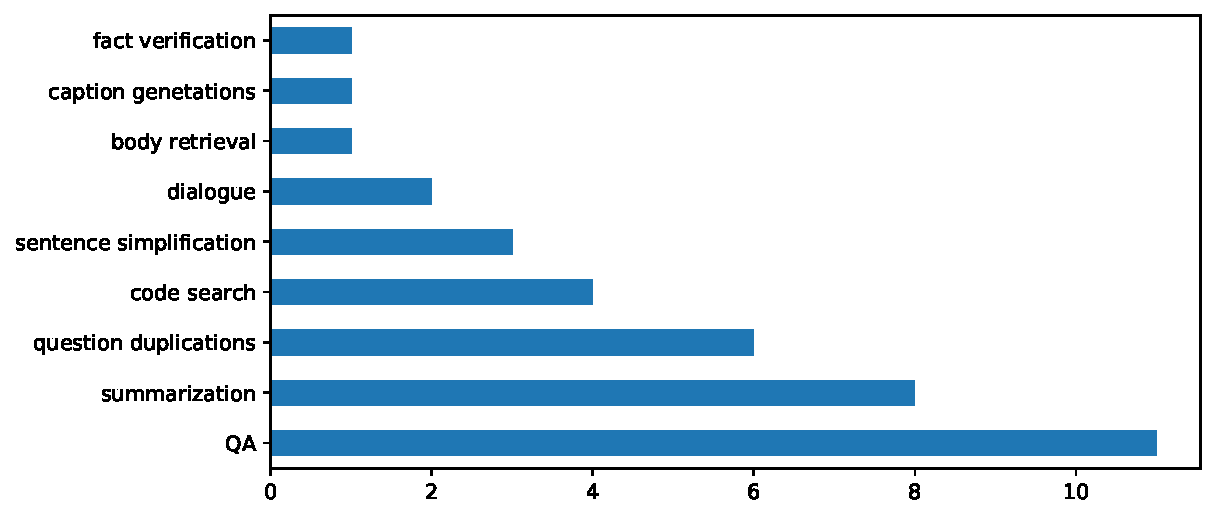
\includegraphics[width=8cm]{imgs/task_stats.pdf}\caption{The task distributions of the datasets included in \rib. 
} \label{fig:task_dist}
\end{figure}
\begin{figure}[t!]
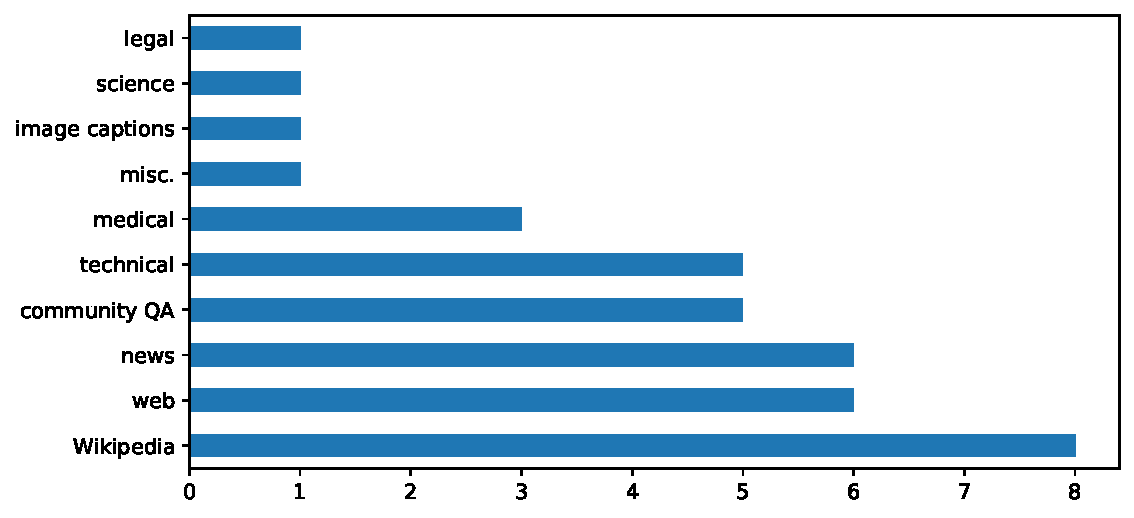
\includegraphics[width=8cm]{imgs/domain_stats.pdf}\caption{The domain distributions of the datasets included in \rib. 
} \label{fig:domain_dist}
\end{figure}

\section{Further Detail about the \task evaluation}
\paragraph{Query and corpus creations.} 
For AmbigQA, we use the official development split, including 1,172 queries, as the official test split annotations are not publicly available.  
We use all paraphrased questions for all train and development sets to form the retrieval corpus. 
For WIKIQA, we combine the development split and test split available at the huggingface datasets,\footnote{\url{https://huggingface.co/datasets/wiki_qa}} and we use the question and answer sentence pairs that are labeled as \texttt{1} as the queries for evaluations, and use the answer sentences as the gold documents.
Regarding the retrieval target, we use all sentences available in the WIKIQA dataset, including the sentences that are labeled as \texttt{0}.   
For LinkSO, we use the original datasets' test split for the python domain and sample 1,000 queries.\footnote{\url{https://sites.google.com/view/linkso}}
We find questions that are labeled as duplicated and use their corpus as our retrieval target. 
For GooAQ-technical, we sample 1,000 GooAQ questions whose answers are from \texttt{stackoverflow.com}. As 20\% of the sampled GooAQ tech queries share the same answer posts, we remove the duplicated paragraphs. 
For CodeSearchNet-Python, we use the comments describing the codes as queries and the corresponding python codes as positive documents. We sample 1,000 queries from the test split. 


\paragraph{Examples.}
Examples of \task are shown in Table~\ref{tab:cross_task_eval_examples}. 
As shown, queries themselves often do not fully indicate the users' intents. 
By specifying users' intents as explicit textual instructions, our model can  effectively perform multi-task retrieval over a single pooled corpus.  
\paragraph{Human evaluations of quality. }
{To access the possibility of having false negative passages, we run an off-the-shelf retrieval system to retrieve the top 10 documents for randomly sampled 20 questions for each task, and we evaluate if any of the negative passages, especially from the non-target corpus, are indeed positive. 
We found that the false negative ratio is less than 10\%. }


\section{Modeling Details}
\subsection{Hyperparameters of \model }
\label{sec:hyperparameters}
\paragraph{\model-dual.}
We set the learning rate to be $1 \times 10^{-5}$ and warm-up steps to be 1,000. The softmax temperature is set to 0.05. 
The batch size is 1024. 
We use 7 negative samples per instance; 10\% of the time we use hard negative or instruction-unfollowing negatives, while 90\% of the time we use negative documents that are randomly sampled from the same target corpus. 
The maximum document chunk length is set to 256. 


\paragraph{\model-full.}
To train a cross-encoder using the T0-3B encoder, we set the maximum sequence length to 512 and the batch size to 1, increasing the gradient accumulation steps to 8. 
We set the dropout rate to 0.1 and the learning rate to 1 $\times 10 ^ {-5}$.  


\subsection{Instructions for Evaluations}
Table~\ref{tab:list_of_instructions_beir} lists the instructions used for the BEIR and \task evaluation. 

\subsection{Negative Sampling}
\label{sec:details_of_negative}
\paragraph{Mining instruction-unfollowing samples.}
To sample instruction-unfollowing samples, given a query from a target dataset, we retrieve the top 20 documents from another task's corpus using Contriever-MS MARCO. For instance, given a PubMedQA, a system should not retrieve a document from a Wikipedia paragraph. 
A list of source target task and retrieval corpus combinations is shown in  Table~\ref{tab:inst_unfollowing_list}.

\begin{table*}[t!]
\footnotesize
    \centering
    \begin{tabular}{lll}%|ccccccc}
\toprule
dataset & expected output &instruction-unfollowing corpus\\
\midrule
Gigaword & article summary &Wikipedia paragraph \\
Medical Paragraph Simplification & simplified text of medical cases &Wikipedia paragraph \\
MS MARCO & web answers & OQA questions \\
OQA & similar questions & Yahoo Answers answer \\
PubMedQA & medical paper abstract & Wikipedia paragraph \\
Qrecc & dialogue responses &Wikipedia paragraph \\
Quora & duplicated questions &Wikipedia paragraph \\
sentence compression & simplified sentence & Wikipedia paragraph \\
StackExchange (question$\rightarrow$answer) title &StackExchange answer & StackExchange title \\
StackExchange (title $\rightarrow$title) title & StackExchange title & StackExchange answer \\
Yahoo Answers & Yahoo Answers answer & Wikipedia paragraphs \\
\bottomrule
 \end{tabular}
    \caption{The list of the combinations of the dataset and corresponding {instruction-unfollowing} corpora to mine instruction-unfollowing negative documents. }\label{tab:inst_unfollowing_list}
\end{table*}


\paragraph{Sampling $\boldsymbol{d}^{-}$ for \model-full training.}
Challenging negative samples help a system to effectively learn the task. On the other hand, prior work also shows that it can lead to large performance drops in out-of-domain datasets, and having both randomly sampled negative documents and carefully designed negative documents is a key to building a system that is competitive in both in-domain and out-of-domain retrieval~\cite{ni2021large}.
To effectively combine the negative documents during training, we first combine random samples and hard negative samples, and then we randomly sample 4 negative documents per one positive document. The number of instruction-unfollowing documents, if applicable, is limited to less than 20\% of the negative documents, and we set the maximum number of instruction-unfollowing samples from certain combinations listed in Table~\ref{tab:inst_unfollowing_list} up to 10k. 


\section{Further Results and Analyses}
\subsection{Qualitative Results on \task}
Table~\ref{tab:cross_task_examples} shows the qualitative examples given different instructions on \task, and Table~\ref{tab:comparison} compares \model-full with Contriever MS MARCO. 

\begin{table*}[t!]
\renewcommand{\arraystretch}{1.2}
\setlength{\tabcolsep}{2pt}
\footnotesize
    \centering
    \begin{tabular}{p{4cm}|p{11cm}}%|ccccccc}
\toprule
\multicolumn{2}{l}{\textbf{Query}: how to calculate the distance between two points using longitude and latitude} \\\hline
\textbf{Instruction} & \textbf{Top document}\\\midrule 
 Retrieve an answer post from StackOverflow to this question & SELECT getDistance(lat1,lng1,lat2,lng2) as distance FROM your\_table. Here's a MySQL function that will take two latitude longitude pairs, and give you the distance in degrees between the two points. It uses the Haversine formula to calculate the distance. \\
 Find a similar question asked in StackOverflow & tried implementing formula good two points testing yet code working distance returns. \\\toprule
 \multicolumn{2}{l}{\textbf{Query}: When did the kim family come to power? } \\\hline
\textbf{Instruction} & \textbf{Top document}\\\midrule 
find an answer sentence & Kim came to lead the Soviet-backed North's provisional government, becoming the first premier of its new government, the Democratic People's Republic of Korea (commonly known as North Korea), in 1948. He started the Korean War in 1950 with hopes to reunify the region. (Wikipedia) \\
Find a similar question & When did the kim family come to power in North Korea? (Ambig QA) \\\toprule
  \multicolumn{2}{l}{\textbf{Query}: 10\% of sudden infant death syndrome (SIDS) deaths happen in newborns aged less than 6 months } \\\hline
\textbf{Instruction} & \textbf{Top document}\\\midrule 
retrieve a scientific paper paragraph to verify this & Despite declines in prevalence during the past two decades, sudden infant death syndrome (SIDS) continues to be the leading cause of death for infants aged between 1 month and 1 year in developed countries. Behavioral risk factors identified in epidemiological studies include prone and side positions for infant sleep, smoke exposure, soft bedding, and sleep surfaces, and overheating. (Scientific paper) \\
Find a Wikipedia paragraph to verify this & By definition, SIDS deaths occur under the age of one year, with the peak incidence occurring when the infant is at 2 to 4 months of age. (Wikipedia) \\
\bottomrule
 \end{tabular}
    \caption{Examples of the model's predictions given different instructions with the same query. The queries and documents are from \task. }\label{tab:cross_task_examples}
\end{table*}

\begin{table*}[t!]
\renewcommand{\arraystretch}{1.2}
\setlength{\tabcolsep}{2pt}
\footnotesize
    \centering
    \begin{tabular}{p{7.5cm}|p{7.5cm}}%|ccccccc}
\toprule
\multicolumn{2}{l}{\textbf{Query}: 10\% of sudden infant death syndrome (SIDS) deaths happen in newborns aged less than 6 months.} \\
\multicolumn{2}{l}{\textbf{Instructions}: Retrieve a scientific paper abstract to verify this}\\\hline
\textbf{Contriever} &  \textbf{\model-full}\\
 \textcolor{red}{\xmark} By definition, SIDS deaths occur under the age of one year, with the peak incidence occurring when the infant is at 2 to 4 months of age. This is considered a critical period because the infant's ability to rouse from sleep is not yet mature (Wikipedia paragraph) &  \textcolor{green}{\checkmark} Despite declines in prevalence during the past two decades, sudden infant death syndrome (SIDS) continues to be the leading cause of death for infants aged between 1 month and 1 year in developed countries. Behavioral risk factors identified in epidemiological studies include prone and side positions for infant sleep, smoke exposure, soft bedding, and sleep surfaces, and overheating. (paper)  \\\toprule
\multicolumn{2}{l}{\textbf{Query}: Which city will host the next winter Olympics?}\\
\multicolumn{2}{l}{\textbf{Instructions}: find an answer from Wikipedia}\\\hline
\textbf{Contriever} &  \textbf{\model-full}\\
 \textcolor{red}{\xmark} Where will the next winter Olympics be held 2018? (Ambig question) & \textcolor{green}{\checkmark} The host city for the 2022 Winter Olympics, is Beijing in northern China, elected on 31 July 2015, at the 128th IOC Session in Kuala Lumpur. Beijing will be the first city ever to have hosted both the Summer and Winter Olympics. The 2022 Winter Olympics will take place between 4 and 20 February 2022. (Wikipedia paragraph) \\ \toprule
 \multicolumn{2}{l}{\textbf{Query}: use batch normalization tensorflow}\\
\multicolumn{2}{l}{\textbf{Instructions}: Can you find python code implementing this? }\\\hline
\textbf{Contriever} &  \textbf{\model-full}\\
 \textcolor{red}{\xmark} could use batch normalization tensorflow 
would like use batch normalization TensorFlow since found source code rel noreferrer core ops nn ops cc however find documented different semantics mlp cnn sure exactly bn find method called either c code copied reference  (StackOverflow post) & 
\textcolor{green}{\checkmark} 
\begin{lstlisting}
def batch_norm(inputs, training, data_format):
  outputs = tf.layers.batch_normalization(
      inputs=inputs, axis=1,
      momentum=_BATCH_NORM_DECAY, epsilon=_BATCH_NORM_EPSILON, center=True,
      scale=True, training=training, fused=True)
 return outputs
\end{lstlisting}
      (GitHub code) 
      \\\toprule
      \multicolumn{2}{l}{\textbf{Query}: how many planets is jupiter away from the sun?} \\
\multicolumn{2}{l}{\textbf{Instructions}: Can you find an answer sentence to this question for me?}\\\hline
\textbf{Contriever} &  \textbf{\model-full}\\
 \textcolor{red}{\xmark} Jupiter is the only planet whose barycenter with the Sun lies outside the volume of the Sun, though by only 7\% of the Sun's radius.[80] The average distance between Jupiter and the Sun is 778 million km (about 5.2 times the average distance between Earth and the Sun, or 5.2 AU) (Wikipedia paragraph) &  \textcolor{green}{\checkmark} Jupiter is the fifth planet from the Sun and the largest planet in the Solar System. (Wikipedia answer sentence) \\\toprule
       \multicolumn{2}{l}{\textbf{Query}: Who won the final hoh big brother 20?} \\
 \multicolumn{2}{l}{\textbf{Instructions}: a question similar to this}\\\hline
\textbf{Contriever} &  \textbf{\model-full} \\
\vspace{-0.5cm}
\begin{itemize}
\itemsep-0.2em 
    \item \textcolor{green}{\checkmark} Who won the Final HoH in the American reality show Big Brother 20? (AmbigQA)
    \item \textcolor{green}{\checkmark}  Who won the final vote in the British reality show Celebrity Big Brother 20? (AmbigQA) 
    \item  \textcolor{red}{\xmark} Caleb Reynolds was a castaway on Survivor: Kaôh Rōng; he was medically evacuated from the game, and placed 15th. Nicole Franzel returned as a HouseGuest on Big Brother 18 where she was crowned the winner and became the first female winner to win against a male in the final 2. (Wikipedia paragraph)
\end{itemize}
  &  
  \vspace{-0.5cm}
  \begin{itemize}
\itemsep-0.2em 
\item \textcolor{green}{\checkmark} Who won the final vote in the British reality show Celebrity Big Brother 20? (AmbigQA)
\item \textcolor{green}{\checkmark} Who is left in the American big brother house at the end of season 20? (AmbigQA)
\item \textcolor{green}{\checkmark} Who won the Final HoH in the American reality show Big Brother 20? (AmbigQA)
\end{itemize}
\\
\bottomrule
 \end{tabular}
    \caption{We compare \model-full outputs with the Contriever-MS MARCO~\cite{izacard2022unsupervised} predictions on \task. We show the top one prediction for the first four examples, and show the top three predictions for the bottom examples. \textcolor{green}{\checkmark} mean that the documents follow instructions while \textcolor{red}{\xmark} mean that the documents do not satisfy the instructions. }\label{tab:comparison}
\end{table*}

\subsection{Analysis of Instruction Effectiveness}
\paragraph{Full results of instruction ablations.}
Table~\ref{tab:inst_ablations_full} shows the full BEIR results of ablating instructions in Section~\ref{sec:robustness}, and Table~\ref{tab:cross_task_results_ablations} shows the ones on LOTTE and \task. 
On all of the benchmarks, removing instructions at training or test time largely hurts the performance, indicating the effectiveness of instructions. 

\begin{table*}[t!]
\centering
\small
\addtolength{\tabcolsep}{-2.25pt}  
\begin{tabular}{@{}laa | cccccccccbb}\toprule
 & \multicolumn{2}{|c|}{Using instructions}  &\multicolumn{11}{c}{\textbf{BEIR}}  \\ \midrule
 &  at training & at test &TREC & NFC & FQA & ARG& TOU & DBP & SCD & CLI&SCF & avg. & best  \\\midrule
\model-full & \checkmark &  \checkmark  &{\bf 72.8}  & 34.6 & {\bf 42.0} & {\bf 50.0} & 	{\bf 35.3} & 	46.1 & 	{\bf 18.4} & 	{ 35.2} & 	73.7 & 	{\bf 44.4}	& 5  \\\hline
 \multirow{3}{*}{Ablations}&\checkmark  &  & 61.1 & 	21.9 &  38.4 & 	39.8 & 	23.6& 36.1 & 	15.0 & 	24.7 &	65.2 &  36.2 & 0   \\
 &   &  \checkmark  & 67.6 & 	{ 34.9}  & 	40.6 & 	39.5 & 	20.5 & 	{\bf 47.1} & 	17.5 & {\bf 39.8} & 	{\bf 75.4} & 	42.5 & 3 \\
 & &  & 57.2 & 	{\bf 37.1} & 	41.3 & 	{\bf 50.0} & 	18.3 & 	41.3 & 	18.3 & 	32.5 & 	73.2 & 	41.1 &  2 \\
\bottomrule
\end{tabular}
    \caption{The full results of the instruction ablations on BEIR. TREC, NFC, FQA, ARG, TOU, DBP, SCD, CLI, SCF indicate TREC-COVID, FIQA, NF Corpus, Arguana, Touche-2020, DBPedia, SciDocs, Climate-Fever, and SciFact, respectively. 
    }
    \label{tab:inst_ablations_full}
\end{table*}

\begin{table*}[t!]
\centering
\footnotesize
\addtolength{\tabcolsep}{-2.5pt}  
\begin{tabular}{laa|c|ccccccb}\toprule
 & \multicolumn{2}{|c|}{Using instructions} & LOTTE & \multicolumn{7}{c}{\task} \\
& at training & at test   & & AMB & WQA & SCF & GAT & LSO & CSP & avg.  \\
\midrule
\model-full & \checkmark & \checkmark & {\bf 75.7} & {\bf 90.5} & 52.5 & {\bf 66.2} & {\bf 68.6} & 24.9 & {\bf 51.4} & {\bf 59.1} \\\hline
 \multirow{3}{*}{Ablations}& \checkmark & & 68.5 & 59.3 & {\bf 54.4} & 61.7 & 62.0 & 15.1 & 46.8 & 49.9 \\
  & & \checkmark & 70.5 & 40.1 & 47.2 & 64.0 & 69.5 & {\bf 25.5} &  43.7 & 48.3 \\
  & &  & 69.9 & 34.5 & 32.5 & 60.8 & 58.2 & 24.2 & 49.3 & 43.3  \\
\bottomrule
\end{tabular}
    \caption{: Instruction ablations on LOTTE (Search pooled) and \task (pooled) evaluation. AMB,
WQA, SCF, GAT, LSO, CSP denotes AmbigQA, WikiQA, SciFact, GooAQ-Technical, LinkSO-Python, and CodeSearchNet-Python, respectively.  
    }
    \label{tab:cross_task_results_ablations}
\end{table*}


\paragraph{Examples of prompts with performance.}
Table~\ref{tab:prompt_performance_full_list} shows the instructions and \model-full performance on three BEIR datasets.  
We also provide a comparison of the model performance when uninformative instructions are given in Table~\ref{tab:prompt_performance}. 
We see that more informative and related instructions often result in a strong performance, while irrelevant instructions degrade it. 

\begin{table*}[t!]
\renewcommand{\arraystretch}{1.2}
\setlength{\tabcolsep}{2pt}
\footnotesize
    \centering
    \begin{tabular}{lp{9cm}r}%|ccccccc}
\toprule
\textbf{Dataset} & \textbf{Instruction} & \textbf{NDCG@10}\\\midrule
\multirow{7}{*}{SciFact} &  \texttt{Find a scientific paper sentence to verify this questions} & 75.4 \\
 & \texttt{Retrieve a scientific paper abstract to verify this claim} & 75.7\\ 
  &\texttt{can you retrieve reliable scientific evidence to check if the following claim is true or not?} &  74.3 \\
  &  \texttt{please retrieve evidence for me to verify the following} &  73.8 \\
   &     \texttt{a scientific paper sentence supporting or refuting the following statement} &  74.7 \\
    \hline
\multirow{5}{*}{Touche-2020} &\texttt{retrieve an argument paragraph to answer this question} & 30.6 \\
&\texttt{retrieve a paragraph to answer this debate question} & 30.9 \\
&\texttt{Find a opinion to this debate question} & 29.5 \\
&\texttt{retrieve an argument paragraph that supports this debate question to this debate question} & 31.2 \\\hline
\multirow{8}{*}{Climate-FEVER} &  \texttt{Retrieve a scientific paper abstract to verify the following claim} &29.3 \\
& \texttt{Retrieve a Wikipedia paragraph to answer this question} & 30.4 \\ 
 & \texttt{Retrieve a Wikipedia paragraph to verify the following claim about climate change} &  30.8 \\
 &   \texttt{I want to know if the following claim is true or not. Can you find Wikipedia evidence?} & 30.6 \\
  &      \texttt{Find a Wikipedia paragraph to verify the following claim} & 30.8 \\
\bottomrule
 \end{tabular}
    \caption{Performance on SciFact, Climate-FEVER and Touche-2020 with different instructions. }\label{tab:prompt_performance_full_list}
\end{table*}


\begin{table*}[t!]
\renewcommand{\arraystretch}{1.2}
\setlength{\tabcolsep}{2pt}
\footnotesize
    \centering
    \begin{tabular}{lp{10cm}r}%|ccccccc}
\toprule
\textbf{Dataset} & \textbf{Instruction} & \textbf{NDCG@10}\\\midrule
\multirow{3}{*}{SciFact} & \textcolor{green}{\checkmark} \texttt{Retrieve a scientific paper abstract to verify this claim} & 75.7 \\
 & \textcolor{red}{\xmark}  \texttt{Retrieve a {Wikipedia paragraph} to verify the following claim} & 74.0 \\
 & \texttt{[NULL]} & 69.1 \\\hline
\multirow{3}{*}{Arguana} & \textcolor{green}{\checkmark} \texttt{Retrieve an article that contradict the following paragraph} & 50.6 \\
 & \textcolor{red}{\xmark} \texttt{Retrieve {a Wikipedia paragraph that answers this question}} & 47.3 \\
 & \texttt{[NULL]} & 39.8 \\\hline
\multirow{3}{*}{Touche-2020} & \textcolor{green}{\checkmark} \texttt{Retrieve an argument for this topic} &29.6 \\
 & \textcolor{red}{\xmark} \texttt{retrieve a Wikipedia passage that answers this question} &26.7 \\
 & \texttt{[NULL]} & 22.1 \\
\bottomrule
 \end{tabular}
    \caption{Full list of the instructions used for evaluations. \texttt{[NULL]} means that at inference time, no instruction is given to \model-full. \textcolor{green}{\checkmark} means a correct instruction, while  \textcolor{red}{\xmark}  means incorrect instructions. }\label{tab:prompt_performance}
\end{table*}


\subsection{Analysis on Model and Dataset Scale}
Table~\ref{tab:beir_scale} shows the NDCG@10 across different model scales. 
We compare the \model-full initialized with different sizes of T5-LM-adapt for a fair comparison. 
We see in general that larger models perform better. 

Table~\ref{tab:dataset_scale_beir} shows the full BEIR results of \model-full trained on varying numbers of datasets. 
We see that as we increase the number of datasets used during training, model performance often improves, which is consistent with previous work on instruction-tuning in LLMs~\cite{wang2022benchmarking}. 



\begin{table*}[t!]
\centering
\small
\addtolength{\tabcolsep}{-2.25pt}  
\begin{tabular}{@{}l|a| cccccccccbb}\toprule
 & model size   &\multicolumn{11}{c}{\textbf{BEIR}}  \\ \midrule
 pretrained models &&TREC & NFC & FQA & ARG& TOU & DBP & SCD & CLI&SCF & avg. & best  \\\midrule
T5-LM-base&110M & 62.9 & 29.7 & 33.9 & 	37.8 & 30.8 & 38.6 & 15.1& 	29.2 & 	70.7 &  38.7 & 0\\
T5-LM-large & 385M & {\bf 73.3 }& {\bf 34.2} & 40.2 & {\bf 47.1} & 32.8 & 45.3 & 18.2 & 35.2 & 74.9 & 43.7	& 3  \\
T5-LM-XL &1.5B & 71.6 & 33.1 & {\bf 41.8} & 43.1 & {\bf 34.0} & {\bf 46.0 }& {\bf 18.5} & {\bf 38.3} & {\bf 75.5} & {\bf 44.7} & {\bf 6}	 \\
\bottomrule
\end{tabular}
    \caption{Zero-shot retrieval results for different sizes of \model-full on BEIR. TREC, NFC, FQA, ARG, TOU, SCD, CLI, SCF indicate TREC-COVID, FIQA, NF Corpus, Arguana, Touche-2020, DBPedia, SciDocs, Climate-Fever, and SciFact, respectively. 
    }
    \label{tab:beir_scale}
\end{table*}
\begin{table*}[t!]
\centering
\small
\addtolength{\tabcolsep}{-2.25pt}  
\begin{tabular}{@{}l|a| cccccccccbb}\toprule
 & dataset number   &\multicolumn{11}{c}{\textbf{BEIR}}  \\ \midrule
  pretrained models& &TREC & NFC & FQA & ARG& TOU & DBP & SCD & CLI&SCF & avg. & best  \\\midrule
% T0-3B &1.5B & 74.3 & 37.2 & 	47.0 & 	50.6 & 	29.6 & 	46.1 & 	18.7 & 	20.5 & 	76.3 & 	{\bf 44.1}	 \\ 
T5-LM-XL &5 & 63.3 & 28.3 & 37.6 & 	47.8 & 24.3 & 42.3 & 17.0 & 30.8 & 	73.4 &   40.5  & 0 \\
T5-LM-XL & 10 & 68.8 & 30.5 & 39.5 & 47.5 & 29.4 & {\bf 46.7} & {\bf 18.2} &  26.9 & {\bf 76.0} &  42.6& 3 \\
T5-LM-XL &20 & 	{\bf 71.0 }& {\bf  33.7} & {\bf 41.7} & {\bf 48.7} & {\bf 33.2} & 46.1 & {\bf 18.2} & {\bf 29.8} & 74.7 & {\bf 44.1} & {\bf 6 } \\
\bottomrule
\end{tabular}
    \caption{Zero-shot retrieval results for different training dataset scales of \model-full on BEIR. TREC, NFC, FQA, ARG, TOU, SCD, CLI, SCF indicate TREC-COVID, FIQA, NF Corpus, Arguana, Touche-2020, DBPedia, SciDocs, Climate-Fever, and SciFact, respectively. 
    }
    \label{tab:dataset_scale_beir}
\end{table*}

\subsection{Analysis on Different Pre-trained Models}
Our \model-full is initialized with the T0-3B encoder. 
We experiment with more recent pretrained instruction-following models: FLAN-T5-XL~\cite{flan_palm} and Tk-Instruct~\cite{wang2022benchmarking}, which are trained on the order of magnitude of more datasets. 
We analyze \model-full performance when we initialize encoders using different pre-trained encoder models, including the ones that are released recently. 
Table~\ref{tab:diff_enc} shows the results of \model-full, when the encoder is initialized with three different recent instruction-following pretrained models, T0-3B, FLAN-T5-XL~\cite{flan_palm} and Tk-Instruct-3B~\cite{wang2022benchmarking}. 
FLAN-T5 shows the best average BEIR performance, outperforming TART-full by 0.7 NDCG@10. 
Tk-Instruct shows a notable performance drop on some datasets (e.g., TREC COVID), resulting in slightly lower performance than the original \model-full (T0-3B). 

\begin{table*}[t!]
\centering
\small
\addtolength{\tabcolsep}{-2.25pt}  
\begin{tabular}{@{}l|cccccccccb}\toprule
  &\multicolumn{10}{c}{\textbf{BEIR}}  \\ \midrule
 pretrained models &TREC & NFC & FQA & ARG& TOU & DBP & SCD & CLI&SCF & avg.   \\\midrule
T0-3B  & 71.7 & {\bf 34.0} & {\bf 42.2} & 	49.8 & 	{\bf 31.2} & 	45.1 & 	17.5 & 	{30.0} & 	75.8 & 	{ 44.1} \\
FLAN-T5 & { 72.8} & 33.4 & 41.8 & { 51.5} & 24.9 & {46.8} & { 18.7} & {\bf  35.4} & {\bf 77.7} & {\bf 44.8}		 \\
Tk-Instruct &  65.4 & 34.7 & 32.3 & 44.5 & 24.3 & 42.3 & 19.2 & 34.0 & 76.2 & 41.4 \\
\bottomrule
\end{tabular}
    \caption{Zero-shot retrieval results for \model-full initialized using different pretrained models on BEIR. TREC, NFC, FQA, ARG, TOU, SCD, CLI, SCF indicate TREC-COVID, FIQA, NF Corpus, Arguana, Touche-2020, DBPedia, SciDocs, Climate-Fever, and SciFact, respectively. 
    }
    \label{tab:diff_enc}
\end{table*}
